% Draft of the body. Article class with natbib for drafting; to be moved to the
% Springer Nature template (sn-jnl) before submission.
\documentclass[11pt]{article}
\usepackage[margin=1in]{geometry}
\usepackage[T1]{fontenc}
\usepackage{lmodern}
\usepackage{amsmath,amssymb}
\usepackage{booktabs}
\usepackage{graphicx}
\usepackage{tikz}
\usetikzlibrary{positioning,arrows.meta,fit}
\usepackage{pgfplots}
\pgfplotsset{compat=1.18}
\usepgfplotslibrary{groupplots}
\usepackage[authoryear,round]{natbib}
\usepackage[hidelinks]{hyperref}
\usepackage{siunitx}

\newcommand{\Sref}[1]{Online Resource~S#1}
\newcommand{\hmmthree}{\textsc{hmm3}}
\newcommand{\hmmten}{\textsc{hmm10}}
\newcommand{\arone}{\textsc{ar1}}
\newcommand{\artwo}{\textsc{ar2}}
\newcommand{\arthree}{\textsc{ar3}}

\title{Per-person sequence models of keystroke behaviour:\\ what remains of the gain against stronger comparisons}
\author{Mikoto Miura\\ Independent Researcher}
\date{Draft, November 2026}

\begin{document}
\maketitle

\begin{abstract}
Claims that a user model fitted to one person beats a shared one depend on what it is compared with. We examined this for sequence models of keystroke behaviour, using keystroke logs symbolized once per second over overlapping 30-second windows from two public datasets: co-writing sessions (CoAuthor) and programming assignments (a CS1 course). We compared per-person fits on later data from the same person with a shared model of the same structure fitted without that person and with the person's own first-order Markov chain, and chose the model structure and the strength of shrinkage toward the shared model on other people. In CoAuthor a per-person three-state hidden Markov model beats a shared model of the same structure by up to 0.19 nats per symbol, but that structure loses to the person's own Markov chain. With a stronger structure on both sides the gain mostly disappears. Once structure and shrinkage are chosen on other people, the person's data carry at most about 1\% of the weight in the chosen fit in the 15-session panel (about 3\% at its largest training size), and the remainder over the shared model is about as large as the gain of a less-smoothed shared model that uses none of the person's data; the protocol cannot attribute it to the person. In CS1, where most symbols are pause seconds, the shared model itself is chosen. For adaptive systems that decide for a whole panel whether to model each person, we suggest comparing with the person's own Markov chain and a same-structure shared model, and reporting the smallest planted difference such a check detects.
\end{abstract}

\noindent\textbf{Keywords:} personalization; user modelling; keystroke logs; hidden Markov models; evaluation protocol; baselines

% ---------------------------------------------------------------------------
\section{Introduction}\label{sec:intro}

Adaptive systems that read behaviour logs often model each person separately: a model fitted to one learner's or writer's own history is expected to describe that person better than a model shared across people. Whether this is worth the cost of collecting enough data per person, of storing a model per person and of a cold start for every newcomer is usually judged by comparing the per-person model with a shared one. That comparison has two sides, and the size of the gain depends on both. A per-person model can look strong because the shared model it is compared with is weak, or because the per-person model repairs a structure that is too simple for the data, and not because people differ in a way the model captures.

This concern is known in other domains. Comparisons with a population baseline rather than with the person's own average make mood and stress models look better than they are \citep{DeMasi2017}, record-wise splits that mix a person's days between training and test inflate accuracy \citep{Saeb2017}, and reports of large per-person gains often compare with a single general model \citep{Weiss2012,Taylor2020,Meegahapola2022}. For sequence models of keystroke behaviour, which estimate a writer's work state from keystroke features over a rolling window and update every few seconds \citep{Uto2020}, we found in our search (\Sref{1}) no study that compared a per-person model with both a stronger shared model and the person's own simple baseline on the person's later data.

We ran this comparison on two public keystroke datasets, symbolized once per second over overlapping 30-second windows. On later data from the same person, we compared per-person fits with a shared model of the same structure fitted without that person and with the person's own first-order Markov chain, and we chose the model structure and the strength of shrinkage toward the shared model on other people. Figure~\ref{fig:scheme} shows which units enter each fit and each choice.

The answer in one sentence: in CoAuthor, a per-person three-state hidden Markov model (HMM) beats a shared model of the same structure by up to 0.19 nats per symbol, but that structure loses to the person's own Markov chain, and once a stronger structure and the shrinkage are chosen on other people, what remains over the shared model is a small amount that the protocol cannot attribute to the person. This changes what a designer can conclude from a per-person gain: a gain over a weak shared model, or a per-person fit that does not beat the person's own Markov chain, says little about whether modelling each person is worth it.

Our contribution is an evaluation protocol for per-person gains in sequence models of keystroke behaviour and what it changes in one case: the gain that a weak comparison shows shrinks, against a stronger one, to a remainder that the protocol cannot attribute to the person (Sections~\ref{sec:res-hmm}--\ref{sec:res-mode}). The protocol combines established parts (selection that does not use the evaluation data, assessment of an individual on other people, interpolation weights chosen on other users, Section~\ref{sec:related}); what we add is its application to per-person sequence models of keystroke behaviour, with the person's own Markov chain as a comparison model and the shared model's prior mode as a diagnostic of how much the shared model's smoothing matters. The results are exploratory and the positive instance rests on one dataset (Section~\ref{sec:limits}). The recommendations are previewed here and stated in full in Section~\ref{sec:discussion}: compare per-person sequence models with the person's first-order Markov chain and with a same-structure shared model, choose structure and shrinkage on other people, and report the smallest planted difference such a check detects at the panel's record length.

% ---------------------------------------------------------------------------
\section{Related work}\label{sec:related}

\paragraph{Per-person gains and their comparisons.}
Reported per-person gains range from small to large, and the size tracks the comparison. In an idiographic stress study, a person-mean baseline beat every general model for 89\% of participants, although for 80\% at least one personal model beat it \citep{Aalbers2023}; individualized knowledge tracing improves on the population model by small amounts \citep{Yudelson2013,Khajah2016}. Large gains have been reported against a single general model, or with splits that mix a person's days across training and test \citep{Weiss2012,Taylor2020,Meegahapola2022}. Record-wise splits can inflate accuracy, and which split fits depends on the use case \citep{Saeb2017,Little2017}. When per-person models overtake pooled ones depends on the domain and the amount of data: a personal mood model overtook a hybrid after about 30 days \citep{LiKamWa2013}, and pooled models beat person-specific ones in experience-sampling data \citep{Leenaerts2024}. Comparisons with a population baseline rather than the person's own average make mood models look better than they are \citep{DeMasi2017}.

\paragraph{Keystroke-based user models.}
Learner-dependent HMMs have been fitted to keystroke features computed over 30-second frames with a 10-second step to analyse writing processes \citep{Uto2020}.
% OPEN: the evaluation design of Uto et al. (2020) is not yet checked in the full text; do not describe it until checked.
In keystroke dynamics, per-person HMMs of keystroke timing improve when conditioned on the key sequence, with frequency-dependent smoothing and backoff toward less specific contexts \citep{Monaco2018}.

\paragraph{Selection and assessment on other people.}
Selection must not use the evaluation data \citep{Cawley2010,Varma2006}, and the prediction error for a target individual can be estimated by predicting each individual from the other $n-1$, which is robust but less relevant to the target \citep{LiuMeng2016}. Choosing interpolation weights on other users and testing on the same users' later text is the practice in personalized keyboard language models \citep{Fowler2015,Shao2020,Adhikary2023}; we do not claim it as new.

\paragraph{Adaptation, pooling and smoothing.}
Our per-person fit is a maximum a posteriori (MAP) adaptation toward a shared model, as in speaker adaptation \citep{Gauvain1994,Reynolds2000}, not a multilevel HMM with person-level random effects \citep{Altman2007,AartsHaslbeck2025}. Choosing the shared model itself (full pooling) on other people is a predictive choice among fixed candidates, not a boundary estimate of a variance component \citep{MorrisLysy2012,Chung2013}.

\paragraph{Sequence-model misfit and Markov baselines.}
Within-data comparisons of an HMM and a first-order Markov chain by DIC have been reported \citep{Shirley2010}; autoregressive HMMs repair within-state autocorrelation \citep{Stoye2025}; first-order chains suffice for web navigation at the page level but not at the topical level \citep{Singer2014}; and information criteria tend to choose too many states \citep{Pohle2017}.
The AR(1)-HMM we use, in which a hidden chain selects which of several transition matrices among the observed symbols is active, is the first-order case of the double chain Markov model; that model, and the mixture transition distribution that reduces the parameters of its higher-order versions, are reviewed by \citet{BerchtoldRaftery2002}.
These comparisons are made within the data used for fitting; we compare on later data from the same person. A search record and a table of prior evaluation designs are in \Sref{1}.

% ---------------------------------------------------------------------------
\section{Data, models and evaluation}\label{sec:methods}

\subsection{Data}\label{sec:data}
CoAuthor contains keystroke logs of writers composing stories and essays with a language-model assistant, in sessions of about 11 minutes \citep{Lee2022}. CS1 is the 2021 release of keystroke data from an introductory programming course \citep{Edwards2023}; a writer's unit there is an assignment, split into work blocks at gaps of 30 minutes or more. Both are public; no new participants were recruited. A writer's units (sessions or assignments) are ordered in time. The 15-session panel contains the CoAuthor writers with at least 20 sessions (17 writers), the 30-session panel those with at least 35 (9 writers), and the CS1 five-assignment panel the students with at least six assignments (23 writers); each panel is named by the largest number of training units it uses. All-writer panels are reported in \Sref{4}.

Table~\ref{tab:data} gives the counts and one property that matters for reading CS1: the share of evaluation symbols at seconds with no key press in the preceding 30 seconds. It is about 5\% in CoAuthor and 72\% in CS1, so the CS1 measure is mostly the prediction of pause seconds. We use CS1 as a boundary case in which the protocol picks the shared model itself.

\begin{table}[t]
\centering
\caption{Panels and evaluation symbols. Pause share: share of evaluation symbols at seconds with no key press in the preceding 30\,s (all writers pooled; per-writer median and quartiles in brackets). Training symbols are per-writer medians.}
\label{tab:data}
\small
\resizebox{\textwidth}{!}{%
\begin{tabular}{lrrrrl}
\toprule
Panel & Writers & $k$ (training units) & Training symbols & Evaluation symbols & Pause share \\
\midrule
CoAuthor, 15-session & 17 & 1--15 & 624--9,673 & 3,296 & 0.046 (0.029 [0.015, 0.046]) \\
CoAuthor, 30-session & 9 & 1--30 & 642--19,427 & 3,318 & 0.042 (0.030 [0.011, 0.046]) \\
CS1, five-assignment & 23 & 1--5 & 16,361--70,395 & 10,635 & 0.716 (0.727 [0.498, 0.841]) \\
\bottomrule
\end{tabular}}
\end{table}

\subsection{Symbol sequences}\label{sec:symbols}
Every second, five keystroke features are computed over the key events of the preceding 30 seconds (median flight time, share of deletions, mean burst length, number of pauses of 2\,s or more, and share of deletions followed by such a pause), combined into two composite values, smoothed exponentially and mapped to a $5\times5$ grid, with one further symbol for the first typing second after a long run of deletions: 26 symbols, one per second. Every step uses only past key events and fixed constants. We use this form because keystroke features over a rolling 30-second window are the input of work-state models that update every few seconds \citep{Uto2020}, so the results speak to models that read keystrokes in this form. The quantization, the features and the public symbolization kit are described in \Sref{2}.

\subsection{Models and comparison models}\label{sec:models}
\paragraph{Structures.} \hmmthree{} and \hmmten{} are HMMs with 3 and 10 hidden states and a categorical emission per state (83 and 349 free parameters). \arone, \artwo{} and \arthree{} are AR(1)-HMMs with 1 to 3 hidden states, in which each state has its own first-order transition matrix among the symbols (675, 1,353 and 2,033 free parameters); \arone{} is a first-order Markov chain. Equations, priors, EM and initialization are in \Sref{3}.

\paragraph{Use case.} A new person's later units are predicted after $k$ of the person's units have been observed, with a shared model fitted before the person arrived. The shared model is refitted without the target writer. This simulates the use case for the fit and the evaluation, but not for the choice: the choice uses other writers' results, whose shared models include the target writer's non-held-out units (Figure~\ref{fig:scheme}).

\paragraph{Shared model.} The same structure is fitted by MAP on all units of all other writers except their evaluation units (writers outside the panel included), with a weak base prior (fixed pseudo-counts in every cell). The strength of this base smoothing was fixed, not chosen on other people. We write $\bar S$ for the shared model's expected counts per symbol, which sum to 1 within each parameter group.

\paragraph{Per-person fit.} The per-person fit is a MAP estimate on the person's $N$ training symbols whose prior pseudo-counts are the base pseudo-counts plus $\tau\bar S$. The person's weight in the posterior is about $N/(N+\tau)$, varying by row with the row's frequency. As $\tau$ grows the fit approaches the normalized $\bar S$ without the base pseudo-counts, which we call the shared model's \emph{prior mode}, and not the shared model itself; $\tau=\infty$ in the grid denotes the shared model itself, a separate candidate. The grid of $\tau$ runs from 0 to $10^6$ (\Sref{8}). The sequence models have no person-level intercept.

\paragraph{Prior mode (diagnostic).} The prior mode uses none of the person's data. It can give zero probability to a symbol pair the other writers never produced; per-person minus mode is then $+\infty$ for that writer, and such writers are counted separately. It is not a candidate in the main analysis; this diagnostic is specific to this prior form.

\paragraph{The person's first-order Markov chain.} Transition counts from the person's training symbols, with $0.5$ added to every cell.

\paragraph{Choice on other people.} For a target writer, the pair of structure and $\tau$ is chosen by the best median, over the other writers of the same panel and $k$, of their own per-person minus chain difference on their evaluation units; ties go to the earlier candidate in an order from the shared model itself through decreasing $\tau$ and, within one $\tau$, from fewer to more free parameters (\Sref{3}). Within the final protocol the target writer's evaluation units enter no fit and no choice. This objective was fixed in the first analysis; it is not the target writer's predictive accuracy. Any optimism from choosing among candidates falls on the per-person minus chain difference, which is the objective, more than on the per-person minus shared difference. A choice by the mean of other writers' held-out log-likelihood is reported as a check (Section~\ref{sec:res-mode}).

\paragraph{Rows of the main table.} The joint choice of structure and $\tau$ (main row); structure fixed at \hmmthree{} and at \arthree{} with $\tau$ chosen (structure-only contrast); and \arone{} against the person's chain (shrinkage-only contrast).

\begin{figure}[t]
\centering
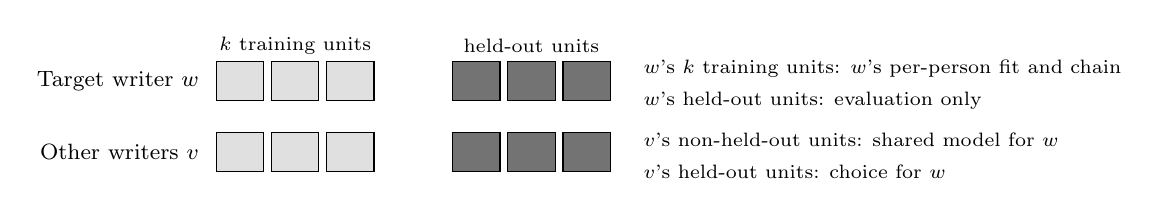
\begin{tikzpicture}[
  unit/.style={draw, minimum width=6mm, minimum height=5mm, inner sep=0pt},
  tr/.style={unit, fill=black!12}, ev/.style={unit, fill=black!55},
  lab/.style={font=\footnotesize, anchor=east}, note/.style={font=\scriptsize, align=left, anchor=west}]
  \node[lab] at (0.6,0) {Target writer $w$};
  \foreach \x in {1.0,1.7,2.4} \node[tr] at (\x,0) {};
  \node[font=\scriptsize] at (1.7,0.45) {$k$ training units};\node[font=\scriptsize] at (4.7,0.45) {held-out units};
  \foreach \x in {4.0,4.7,5.4} \node[ev] at (\x,0) {};
  \node[lab] at (0.6,-0.9) {Other writers $v$};
  \foreach \x in {1.0,1.7,2.4} \node[tr] at (\x,-0.9) {};
    \foreach \x in {4.0,4.7,5.4} \node[ev] at (\x,-0.9) {};
  \node[note] at (6.0,0.15) {$w$'s $k$ training units: $w$'s per-person fit and chain};
  \node[note] at (6.0,-0.25) {$w$'s held-out units: evaluation only};
  \node[note] at (6.0,-0.75) {$v$'s non-held-out units: shared model for $w$};
  \node[note] at (6.0,-1.15) {$v$'s held-out units: choice for $w$};
\end{tikzpicture}
\caption{Which units enter each fit and each choice. Light: training units; dark: held-out units. The shared model for $w$ uses all other writers' units except their held-out units (including writers outside the panel). The choice for $w$ uses the other writers' per-person minus chain differences on their held-out units; their shared models include $w$'s non-held-out units. The target writer's held-out units enter no fit and no choice.}
\label{fig:scheme}
\end{figure}

\subsection{Evaluation and status of the analyses}\label{sec:eval}
For each writer, the held-out units are the last five sessions (CoAuthor) or the last assignment (CS1), and the training units are the $k$ units immediately preceding them (extending back in time as $k$ grows). Each held-out unit is scored as its own sequence, one step ahead. The measure is nats per symbol: per writer, the total log-likelihood over held-out symbols divided by their number. We report, over writers, the median of the per-writer difference, its interquartile range, the share of writers favouring the per-person fit and $n$; intervals are percentile bootstrap intervals that resample writers with their values fixed, without refitting or re-choosing (\Sref{7}).

The study consists of four analyses designed one after another and five later checks (\Sref{12}). For each, the conditions (rows, grids, readings) were committed before its code or, for reanalyses of stored values, before its computation; changes after seeing results are listed in \Sref{12}. All analyses are descriptive: we use no significance tests and no threshold for a meaningful difference. The verification record (self-tests, mutation checks, reproduction checks) is in \Sref{11}.

% ---------------------------------------------------------------------------
\section{Results}\label{sec:results}

\subsection{A three-state HMM fitted per person beats a shared model of the same structure in CoAuthor}\label{sec:res-hmm}
We first checked the comparison a typical study makes: a per-person HMM against a shared model of the same structure. With \hmmthree{} fixed and $\tau$ chosen on other people, the per-person fit beats the shared \hmmthree{} in the 15-session panel at every $k$, from $+0.012$ nats per symbol at $k=1$ (10 of 17 writers) to $+0.188$ at $k=5$ (15 of 17) and $+0.165$ at $k=15$ (17 of 17). The chosen $\tau$ is 0 for every writer at $k=5$ and 15, so this per-person fit uses the person's data alone. The 30-session panel shows the same pattern ($+0.165$ at $k=30$, 9 of 9). In CS1 the gain is not consistent ($+0.007$ at $k=1$ and $+0.028$ at $k=5$, about 60\% of writers on the per-person side).

Taken alone, this is the kind of result that would support modelling each person. The next two sections ask what it is a gain over. All structures and $k$, the all-writer panels and \hmmten{} are in \Sref{5}, and a check of whether the per-person fit compensates for a structure that is too simple is in \Sref{14}.

\subsection{The person's first-order Markov chain is a strong baseline}\label{sec:res-chain}
We next compared the per-person fit with the simplest model of the person's own symbols: their first-order Markov chain. \hmmthree{} loses to it for every writer at every $k$ in CoAuthor, and in CS1 for every writer at $k=3$ and 5 and all but one at $k=1$ and 2: per-person minus chain is $-0.48$ to $-0.54$ nats per symbol in the 15-session panel and about $-1.0$ to $-1.1$ in CS1 (\Sref{5}). The shared \hmmthree{} is worse still ($-0.52$ at $k=1$ and $-0.81$ at $k=15$ against the person's chain in the 15-session panel). The structure that showed a large per-person gain in Section~\ref{sec:res-hmm} is thus one that cannot carry the dependence between consecutive symbols.

A model check points the same way. One-step-ahead randomized quantile pseudo-residuals \citep{Dunn1996} on the two ordered grid axes (the deletion-run symbol excluded) leave a lag-1 autocorrelation of 0.23 to 0.64 for \hmmthree{} and small values for \arthree{} and the chain (\Sref{13}). The strength of this baseline depends on the symbolization: with non-overlapping windows (direction only) \hmmthree{} beats the chain in CoAuthor (\Sref{13}).

The shrinkage-only row of Table~\ref{tab:main} isolates what shrinkage adds when the structure is the chain itself. \arone{} shrunk toward the shared chain beats the person's chain by $+0.043$ at $k=5$ (17 of 17 writers), falling to $+0.007$ at $k=15$ (13 of 17) (Figure~\ref{fig:k}).

\begin{figure}[t]
\centering
\begin{tikzpicture}
\begin{groupplot}[group style={group size=2 by 1, horizontal sep=1.9cm},
  width=0.42\textwidth, height=5.2cm, xlabel={$k$ (training sessions)},
  xtick={1,2,3,5,8,12,15}, legend style={font=\scriptsize, at={(0.5,-0.32)}, anchor=north, legend columns=2},
  every axis plot/.append style={thick, mark size=1.6pt}, tick label style={font=\scriptsize}, label style={font=\small}]
\nextgroupplot[ymode=log, ylabel={nats per symbol}, title={\footnotesize (a) vs.\ same-structure shared model}]
\addplot table[x=k, y=pp_minus_shared, col sep=comma] {figdata/fig2_p15_hmm3.csv};
\addplot table[x=k, y=pp_minus_shared, col sep=comma] {figdata/fig2_p15_ar1.csv};
\addplot table[x=k, y=pp_minus_shared, col sep=comma] {figdata/fig2_p15_ar3.csv};
\addplot[dashed, mark=o] table[x=k, y=pp_minus_shared, col sep=comma] {figdata/fig2_p15_joint.csv};
\nextgroupplot[ylabel={nats per symbol}, title={\footnotesize (b) vs.\ the person's Markov chain}]
\addplot table[x=k, y=pp_minus_chain, col sep=comma] {figdata/fig2_p15_hmm3.csv};
\addplot table[x=k, y=pp_minus_chain, col sep=comma] {figdata/fig2_p15_ar1.csv};
\addplot table[x=k, y=pp_minus_chain, col sep=comma] {figdata/fig2_p15_ar3.csv};
\addplot[dashed, mark=o] table[x=k, y=pp_minus_chain, col sep=comma] {figdata/fig2_p15_joint.csv};
\legend{\hmmthree{} ($\tau$ chosen), \arone{} ($\tau$ chosen), \arthree{} ($\tau$ chosen), joint choice}
\end{groupplot}
\end{tikzpicture}
\caption{Medians over the 17 writers of the 15-session panel. (a) Per-person minus the same-structure shared model, log scale (all medians are positive). (b) Per-person minus the person's first-order Markov chain. The joint choice selects \arthree{} for every writer and every $k$. Intervals are in \Sref{7}.}
\label{fig:k}
\end{figure}

\subsection{Choosing structure and shrinkage on other people leaves a remainder that the protocol cannot attribute to the person}\label{sec:res-protocol}
We then applied the full protocol: structure and $\tau$ chosen jointly on other people. What we wanted to know was how much of the per-person gain survives when the shared model is given the stronger structure as well.

The protocol picks \arthree, the largest structure in the grid, for every writer in every cell (Table~\ref{tab:main}). Against the person's chain it gains $+0.220$ at $k=1$ falling to $+0.020$ at $k=15$ in the 15-session panel (every writer), and $+0.050$ to $+0.029$ in CS1. Against the same-structure shared model it gains $+4.1\times10^{-4}$ to $+7.2\times10^{-4}$ in the 15-session panel (16 or 17 of 17 writers) and $+1.1\times10^{-3}$ at $k=30$ in the 30-session panel (6 of 9). In CS1 the shared model itself is chosen for every writer, so the difference is zero by construction. The structure-only row shows that most of the per-person \hmmthree{} gain belongs to the weak structure: with \arthree{} on both sides, per-person minus shared is $+5.5\times10^{-4}$ and $+7.6\times10^{-4}$ at $k=5$ and 15, more than two orders of magnitude below the \hmmthree{} gain.

The chosen shrinkage is strong. In the 15-session panel $\tau=10^6$ for every writer at $k=1$ to 12 and $3\times10^5$ for 16 of 17 at $k=15$ (in the 30-session panel, $3\times10^4$ for 8 of 9 at $k=30$). With the median numbers of training symbols, the person's data carry about 0.06\% of the weight at $k=1$, 0.8\% at $k=12$ and 3\% at $k=15$. The chosen fit is therefore close to the prior mode, which leads to Section~\ref{sec:res-mode}.

\begin{table}[t]
\centering
\caption{Main table. Medians over writers of per-writer differences in nats per symbol (share of writers favouring the per-person fit; 95\% bootstrap interval of the median in brackets). Weight: the person's share $N/(N+\tau)$ at the median number of training symbols. The prior-mode columns are diagnostics; ``mode $-$ shared'' does not depend on $k$. $+\infty$ writers are counted in \Sref{9}.}
\label{tab:main}
\scriptsize
\setlength{\tabcolsep}{3pt}
\resizebox{\textwidth}{!}{%
\begin{tabular}{llllllll}
\toprule
Row & Panel, $k$ & Chosen & Weight & Per-person $-$ shared & Per-person $-$ chain & Per-person $-$ mode & Mode $-$ shared \\
\midrule
Joint choice & 15-s., 1 & \arthree, $10^6$ & 0.06\% & $+4.8$e$-4$ (1.00) [3.2e$-4$, 5.9e$-4$] & $+0.220$ (1.00) & $-3.5$e$-4$ (0.18) & $+7.4$e$-4$ (0.88) \\
 & 15-s., 5 & \arthree, $10^6$ & 0.3\% & $+5.5$e$-4$ (1.00) [4.2e$-4$, 6.6e$-4$] & $+0.059$ (1.00) & $-2.8$e$-4$ (0.18) & \\
 & 15-s., 15 & \arthree, $3\times10^5$ & 3\% & $+4.1$e$-4$ (0.94) [2.2e$-4$, 7.8e$-4$] & $+0.020$ (1.00) & $-2.5$e$-4$ (0.35) & \\
 & 30-s., 30 & \arthree, $3\times10^4$ & 39\% & $+1.1$e$-3$ (0.67) [$-2.2$e$-3$, 3.7e$-3$] & $+0.013$ (1.00) & $+5.4$e$-4$ (0.78) & $+7.2$e$-4$ (0.78) \\
 & CS1, 5 & \arthree, $\infty$ & 0 & 0 & $+0.029$ (1.00) & $-2.0$e$-4$ (0.00) & $+2.0$e$-4$ (1.00) \\
\midrule
\hmmthree{} fixed & 15-s., 5 & 0 & 100\% & $+0.188$ (0.88) [0.103, 0.321] & $-0.518$ (0.00) & & $+4.2$e$-5$ (0.94) \\
 & 15-s., 15 & 0 & 100\% & $+0.165$ (1.00) [0.110, 0.302] & $-0.522$ (0.00) & & \\
 & CS1, 5 & $10^3$ (22 of 23) & 99\% & $+0.028$ (0.57) [$-0.039$, 0.053] & $-1.096$ (0.00) & & \\
\midrule
\arthree{} fixed & 15-s., 5 & $10^6$ & 0.3\% & $+5.5$e$-4$ (1.00) [4.2e$-4$, 6.6e$-4$] & $+0.059$ (1.00) & & $+7.4$e$-4$ (0.88) \\
 & 15-s., 15 & $10^6$ & 1\% & $+7.6$e$-4$ (1.00) [6.0e$-4$, 9.5e$-4$] & $+0.020$ (1.00) & & \\
\midrule
\arone{} vs.\ chain & 15-s., 5 & $10^6$ & 0.3\% & $+3.0$e$-4$ (1.00) & $+0.043$ (1.00) [0.033, 0.050] & & $+2.9$e$-4$ (0.88) \\
 & 15-s., 15 & $3\times10^4$ & 24\% & $+0.002$ (0.82) & $+0.007$ (0.76) [0.003, 0.011] & & \\
\bottomrule
\end{tabular}}
\end{table}

How small a difference could this protocol have detected? We planted per-person differences in symbol-to-symbol transitions of synthetic writers matched to the panels, at $10^{-3}$, $3\times10^{-3}$, $10^{-2}$ and $3\times10^{-2}$ nats per symbol, two seeds each. At the CoAuthor record length the protocol detected them from $10^{-2}$ at $k=15$ and only at $3\times10^{-2}$ at $k=5$, and it returned only part of each planted difference; in CS1 it detected them from $10^{-3}$ (\Sref{15}). The real remainder exceeds the largest median of the synthetic negative controls, but in the synthetic writers the prior mode was worse than the shared model, so the negative control did not contain the real smoothing gap and the two are not on the same footing; in synthetic CS1 writers $\tau=10^6$ was mostly chosen rather than the shared model itself (in one negative control 11 of 23 writers chose the shared model), so we do not use the CS1 sensitivity to read the real CS1 panel. The remainder neither shows nor rules out per-person differences (Section~\ref{sec:limits}). The symbolization matters for its size: with unsmoothed symbols per-person minus shared is $+5.8\times10^{-4}$ and $+8.0\times10^{-4}$ at $k=5$ and 15; with non-overlapping windows (direction only) \hmmthree{} is chosen in CoAuthor and the difference stays positive (\Sref{13}).

\subsection{At the chosen shrinkage the per-person fit is close to the prior mode, and the remainder is of the size of the shared model's smoothing gap}\label{sec:res-mode}
Because the chosen fit sits near the prior mode, we compared the prior mode with the shared model directly. For \arthree, prior mode minus shared is $+7.4\times10^{-4}$ in the 15-session panel (15 of 17 writers positive), about the size of the remainder. In the median, then, a version of the shared model with less smoothing, which uses none of the person's data, gains about as much as the per-person fit; it also gives zero probability to the held-out data of 2 of 17 writers, so it is a diagnostic and not a usable model.

Per-person minus prior mode is small and of either sign across panels: $-3.5\times10^{-4}$ to $-1.6\times10^{-4}$ in the 15-session panel (3 to 6 of 17 positive) and $+5.4\times10^{-4}$ at $k=30$ in the 30-session panel (7 of 9) (\Sref{9}). We do not read a direction from it (Section~\ref{sec:limits}). Choosing by the mean of other writers' held-out log-likelihood instead of the median gives the same picture: in the 15-session panel the per-person fit again does not exceed the prior mode ($-3.5\times10^{-4}$ to $-1.2\times10^{-4}$), and the 30-session panel at $k=30$ again does ($+6.0\times10^{-4}$) (\Sref{9}). This comparison of medians does not apportion the remainder between smoothing and the person; a per-writer decomposition did not separate a planted difference from none in synthetic writers (\Sref{15}).

% ---------------------------------------------------------------------------
\section{Discussion}\label{sec:discussion}

A per-person sequence model can be judged only against the comparison it is given. In CoAuthor, the same per-person fitting procedure shows a gain of up to 0.19 nats per symbol against a shared model of a weak structure, and a remainder of about $5\times10^{-4}$ against a shared model of a stronger structure, once structure and shrinkage are chosen on other people; that remainder is of the size that a less-smoothed shared model gains without any of the person's data. For a designer deciding whether to model each person, the first number argues for per-person models and the second gives no reason to, and the difference between them lies in the comparison, not in the people.

\paragraph{What was established and what was not.} Measured: the weak structure loses to the person's own Markov chain, a stronger structure removes most of the gain, and the chosen shrinkage gives the person's data at most about 1\% of the weight in the 15-session panel (3\% at $k=15$; 39\% at $k=30$ in the 30-session panel, where the remainder is $+1.1\times10^{-3}$ for 6 of 9 writers). Not established: whether CoAuthor writers differ in their keystroke sequences in ways the protocol could not detect. The synthetic check bounds what it can detect at this record length, and the remainder is below that bound; it neither shows nor rules out per-person differences.

\paragraph{Scale.} Over one hour of typing at one symbol per second (3,600 symbols), the \hmmthree{} gain over the same-structure shared model corresponds to about 680 nats, and the \arthree{} gain over the person's chain to about 70 to 800, while the remainder in the 15-session panel corresponds to about 1.5 to 2.6 nats and is not shown to be per-person. Sums over overlapping-window symbols are not independent evidence, and we set no threshold for what matters; the comparison concerns predictive accuracy, and downstream benefit and cost were not measured. A per-person logistic model of a proxy label showed the same pattern: it did not beat the person's own base rate (\Sref{10}).

\paragraph{Recommendations.} For studies that decide for a whole panel whether to model each person, and for this kind of symbolization, we recommend what this study evaluated:
(1) compare per-person sequence models with the person's first-order Markov chain and with a shared model of the same structure fitted without the person;
(2) choose structure and shrinkage on other people, with the shared model itself among the candidates;
(3) report, from a synthetic check at the panel's record length, the smallest planted difference the protocol detects;
(4) report the shared model's prior mode next to the result, with the number of writers to whom it gives zero probability, while noting that we have not evaluated whether it measures the effect of smoothing.
Three extensions were not evaluated here: choosing the shared model's base smoothing on other people as well; a separate shrinkage per context, as in frequency-dependent smoothing \citep{Monaco2018}; and a nested design that removes the target person from the other people's shared models. Assessing an individual on other people trades relevance to that individual for robustness \citep{LiuMeng2016}; the protocol makes this trade explicit by deciding for a panel and reporting what it could not detect.

% ---------------------------------------------------------------------------
\section{Limitations}\label{sec:limits}

\begin{itemize}
\item Two datasets and one quantization carry the main results, on overlapping-window symbolizations; the size of what remains depends on the symbolization (Section~\ref{sec:res-protocol}). Sessions and assignments are not days, and the results are not extended to other languages, input methods or populations.
\item In CS1 about 72\% of evaluation symbols are pause seconds (about 5\% in CoAuthor), so the CS1 measure is mostly the prediction of pause seconds; the CS1 evaluation unit is also a different assignment from the training units.
\item Hidden states are not named and are not read as cognitive or affective states, and a better-predicting structure is not read as the true one.
\item No significance tests are used and no threshold defines a meaningful difference; the structure-compensation check (\Sref{14}) and the synthetic check (\Sref{15}) use descriptive rules fixed before their computation. Comparisons of medians are not per-writer decompositions.
\item The analyses were designed one after another after seeing earlier results (\Sref{12}); changes made after seeing results (the $\tau$ grid, the structure families) may favour a smaller remainder. The structure grid stops at three states, and \arthree, its largest structure, was chosen in every cell; a larger shared structure may absorb between-person heterogeneity \citep{Pohle2017}. Second-order smoothed Markov chains and multilevel HMMs were not fitted.
\item The protocol returns only part of a planted difference. At the CoAuthor record length it did not detect planted differences below $10^{-2}$ ($k=15$) or $3\times10^{-2}$ ($k=5$), with four planted levels and two seeds each, and only differences in symbol-to-symbol transitions were planted. A difference planted in 5 of 17 synthetic writers was not detected in the panel median. Neither the remainder nor the sign of per-person minus prior mode shows that per-person differences are absent or present.
\item The strength of the shared model's base smoothing was fixed, not chosen on other people, and the gap between prior mode and shared model reflects that choice. At the chosen $\tau$ the remainder cannot be attributed to the person's data; $10^6$ is the largest finite value of the grid, so the shrinkage choice also sits at the edge. The prior-mode comparison was made on the original symbolization only. The 30-session panel has 9 writers.
\item The choice makes one decision for a whole panel and is not fixed before the target writer arrives; a nested design was not run. The synthetic negative control did not reproduce the real ordering of prior mode and shared model, and synthetic CS1 writers were mostly given $\tau=10^6$ where the real panel chose the shared model itself.
\item Per-person fits reached the same solution from different starts (\Sref{11}), but the dependence of the remainder on the shared model's starting point was not measured. The $0.5$ added to every cell of the person's chain is fixed, and we did not compare with a shared model that includes the target writer's training units.
\item The unsmoothed-symbol check removes the smoothing and, in one variant, the window overlap, but the seconds since the last key press still carry memory across windows (\Sref{13}). Readers can check the symbols only through the public kit's synthetic conformance test until per-record hashes of the original symbol sequences are published.
\end{itemize}

% ---------------------------------------------------------------------------
\section{Conclusion}\label{sec:conclusion}

In CoAuthor, a per-person three-state HMM beats a shared model of the same structure, but that structure loses to the person's own Markov chain; with a stronger structure and shrinkage chosen on other people, what remains is about as large as the gain of a less-smoothed shared model that uses none of the person's data, and the protocol cannot attribute it to the person. Per-person gains in sequence models of keystroke behaviour should be reported against the person's own Markov chain and a same-structure shared model, together with the smallest difference the check can detect.

% ---------------------------------------------------------------------------
\section*{Statements and declarations}
\paragraph{Data availability.} CoAuthor \citep{Lee2022} and the CS1 keystroke data, 2021 release \citep{Edwards2023}, are public; archive links and versions are given in \Sref{2}. No per-writer values of real writers are released; aggregate and synthetic values are.
\paragraph{Code availability.} The symbolization kit; the fitting code (EM, choice of structure and $\tau$, summaries); and the code of the later checks (pseudo-residuals, structure compensation, synthetic sensitivity and its decomposition, the prior mode, the choice objective and the pause share).
\paragraph{Funding.} None.
\paragraph{Competing interests.} The author declares no competing interests.
\paragraph{Ethics.} Public data only; no new participants.

\bibliographystyle{plainnat}
\bibliography{references}

\end{document}
